\chapter{話しことばチェッカーとグレーゾーン\label{c3}}

% 話しことばチェッカー関連

\section{話しことばの定義 \label{c3s1}}
本研究チームにおける「話しことば」の定義は,特に大学初年次の学生が自らレポート推敲が行えることが望ましい非学術的な表現と定義されている.ただし,本研究チームにおいての話しことばは,会話による話し言葉ではなく,レポートや論文などの文章に現れる「書かれた話し言葉」を指す.

\section{話しことばカテゴリ \label{c3s2}}
これまでの研究により,話しことばには,単語そのものが話しことばである表現や,単語の位置関係,例えばある単語の直前にある単語との組み合わせによって話しことばと判断される表現が存在することがわかっている.これらの表現に対し,本研究チームでは「話しことばカテゴリ」と定義している.カテゴリは,表3.1に示すように,前述のような単語の位置関係や品詞などに応じて5つに分類される.

\begin{table}[H]
\centering
\caption{話しことばカテゴリ}
\begin{tabular}{|c|l|l|l|}
\hline
\multicolumn{1}{|c|}{番号} & \multicolumn{1}{c|}{名称} & \multicolumn{1}{c|}{説明} & \multicolumn{1}{c|}{例} \\ \hline
1 & INDEPENDENCE & 対象の単語がある           & \begin{tabular}[c]{@{}l@{}}当たり前、\\あんまり\end{tabular} \\ \hline
2 & PREFIX       & \begin{tabular}[c]{@{}l@{}}対象の単語およびその直前に\\ 特定の品詞の単語がある\end{tabular} & \begin{tabular}[c]{@{}l@{}}名詞+して、\\動詞+して\end{tabular} \\ \hline
3 & SUFFIX       & \begin{tabular}[c]{@{}l@{}}品詞の組み合わせを必要とせず、\\なおかつ複数の単語から成り立つ\end{tabular} & \begin{tabular}[c]{@{}l@{}}くせ+に、\\ かも+しれ+ない\end{tabular} \\ \hline
4 & COLLOCATION  & \begin{tabular}[c]{@{}l@{}}対象の単語およびその単語と\\同じ文章に特定の単語がある\end{tabular} & \begin{tabular}[c]{@{}l@{}}一番+形容詞\\ どうしても+たい \end{tabular} \\ \hline
5 & OTHER   & \begin{tabular}[c]{@{}l@{}}文法的誤り、若者的な言葉遣いなど、\\上記4つ以外に当てはまるもの\end{tabular}  & 全然+違う \\ \hline
\end{tabular}
\label{RJCS-category}
\end{table}

\section{話しことば事例集 \label{c3s3}}
本研究チームが取り扱う話しことばは,日本語教育のエキスパートによる分類によって定められている.分類する際の基準は,大学生向けのレポートの書き方について書かれた関連書籍で示されていることである.過去の研究では,前述の基準で示された話しことばや,初年度教育の講義で学生が作成したレポートなどから話しことばの抽出を行い,話しことば事例集としてまとめた.エキスパートが話しことばを抽出する際に用いた関連書籍の一覧を表\ref{spoken-book}に示す.

\begin{table}[H]
\centering
\caption{「レポートの書き方」関連書籍一覧}
\begin{tabular}{|l|}
\hline
\begin{tabular}[l]{@{}l@{}}創価大学学士課程教育機構(2017)『レポート作成の手引き 2017 年度版』\end{tabular} \\ \hline
\begin{tabular}[l]{@{}l@{}}秋岡伸彦(2007)『文章表現テキスト』東京農業大学出版会\end{tabular}  \\ \hline
\begin{tabular}[l]{@{}l@{}}石黒圭(2012)『この1冊できちんと書ける!論文・レポートの基本』\\ 日本実業出版社\end{tabular}  \\ \hline
\begin{tabular}[l]{@{}l@{}}石坂春秋(2003)『レポート・論文・プレゼンスキルズ』くろしお出版\end{tabular}  \\ \hline
\begin{tabular}[l]{@{}l@{}}井下千以子(2014)『思考を鍛えるレポート・論文作成法〔第 2 版〕』\\慶応義塾大学出版会\end{tabular}  \\ \hline
\begin{tabular}[l]{@{}l@{}}上戸理恵・遠藤郁子・神田由美子・羽矢みずき・藤田和美・与那覇惠子(2016)\end{tabular}  \\ \hline
\begin{tabular}[l]{@{}l@{}}『新編マスター日本語表現〔第 2 版〕』ひつじ書房\end{tabular}  \\ \hline
\begin{tabular}[l]{@{}l@{}}大島弥生・池田玲子・大場理恵子・加納なおみ・高橋淑郎・岩田夏穂(2014)\end{tabular}  \\ \hline
\begin{tabular}[l]{@{}l@{}}『ピアで学ぶ大学生の日本語表現〔第 2 版〕』ひつじ書房\end{tabular}  \\ \hline
\begin{tabular}[l]{@{}l@{}}石井一成著(2011)『ゼロからわかる大学生のためのレポート・論文の書き方』\\ナツメ社\end{tabular}  \\ \hline
\begin{tabular}[l]{@{}l@{}}長尾佳代子・村上昌考(2015)『大学1年生のための日本語技法』ナカニシヤ出版\end{tabular}  \\ \hline
\begin{tabular}[l]{@{}l@{}}銅直信子・坂東実子(2013)『大学生のための文章表現\&口頭発表練習帳』\\ 図書刊行会\end{tabular}  \\ \hline
\begin{tabular}[l]{@{}l@{}}森下稔・久保田英助・鴨川明子編(2010)『新版 理工系学生のための日本語表現法』\\東信堂\end{tabular}  \\ \hline
\begin{tabular}[l]{@{}l@{}}菊田千春・北林利治(2006)『大学生のための論理的に書き、プレゼンする技術』\\ 東洋経済新報社\end{tabular}  \\ \hline
\begin{tabular}[l]{@{}l@{}}伊藤義之(2003)『はじめてのレポート レポート作成のための 55 のステップ』\\ 嵯峨野書院\end{tabular} \\ \hline
\end{tabular}
\label{spoken-book}
\end{table}

% 使用箇所: c3s3

話しことば事例集では,抽出した話しことばに対し,話しことばカテゴリ,その表現が話しことばである理由,書きことばへの修正例を追加情報として付与している.

\begin{table}[H]
\centering
\caption{話しことば事例集から抜粋}
\small % \footnotesize
\begin{tabular}{|c|c|l|l|}
\hline
\multicolumn{1}{|c|}{話しことば} & \multicolumn{1}{c|}{カテゴリ} & \multicolumn{1}{c|}{原文} & \multicolumn{1}{c|}{修正例} \\ \hline
あいにく & INDEPENDENCE & \begin{tabular}[c]{@{}l@{}} 陸上種目の初日は\\あいにくの雨だった. \end{tabular}              & \begin{tabular}[c]{@{}l@{}}陸上種目の初日は\\雨だった.\end{tabular} \\ \hline
当たり前 & INDEPENDENCE & \begin{tabular}[c]{@{}l@{}}水道の水が飲めるのは\\日本だけでは当たり前の\\ことである.\end{tabular} & \begin{tabular}[c]{@{}l@{}}水道の水が飲めるのは\\日本だけでは当然の\\ことである.\end{tabular} \\ \hline
し      & PREFIX       & \begin{tabular}[c]{@{}l@{}}営業時間を退縮すれば,\\客が減るし売り上げも\\減る.\end{tabular}       & \begin{tabular}[c]{@{}l@{}}営業時間を退縮すれば,\\客が減り売り上げも\\減る.\end{tabular} \\ \hline
てる    & PREFIX       & \begin{tabular}[c]{@{}l@{}}犯罪に巻き込まれる危\\険性が指摘されてる.\end{tabular}               & \begin{tabular}[c]{@{}l@{}}犯罪に巻き込まれる危\\険性が指摘されている. \end{tabular} \\ \hline
くせに   & SUFFIX      & \begin{tabular}[c]{@{}l@{}}社会人のくせに名刺の\\渡し方も知らない.\end{tabular}                 & \begin{tabular}[c]{@{}l@{}}社会人でありながら\\名刺の渡し方も知らない. \end{tabular}\\ \hline
てて    & SUFFIX       & \begin{tabular}[c]{@{}l@{}}仕事をしてても SNS \\のこと気になる状態を \\SNS 中毒という.\end{tabular} & \begin{tabular}[c]{@{}l@{}}仕事をしていても SNS \\のことが気になる状態を \\SNS 中毒という.\end{tabular} \\ \hline
一番    & COLLOCATION  & \begin{tabular}[c]{@{}l@{}}家族には一番の味方で\\あってほしいと願うものだ.\end{tabular} & \begin{tabular}[c]{@{}l@{}}家族には最大の味方で\\あってほしいと願うものだ.\end{tabular} \\ \hline
一番に   & OTHER        & \begin{tabular}[c]{@{}l@{}}一番に解決しなければ\\ならない.\end{tabular} & \begin{tabular}[c]{@{}l@{}}初めに解決しなければ\\ならない.\end{tabular} \\ \hline


\end{tabular}
\label{spoken-ex}
\end{table}











\section{話しことばチェッカー \label{c3s4}}
本研究チームで研究および開発・保守を行っている話しことばチェッカーは,文章中に含まれる話しことばを検出し,書きことばへの修正例を提示し,学生自身による推敲をサポートするWebシステムである.

\begin{figure}[H]
	\centering
 	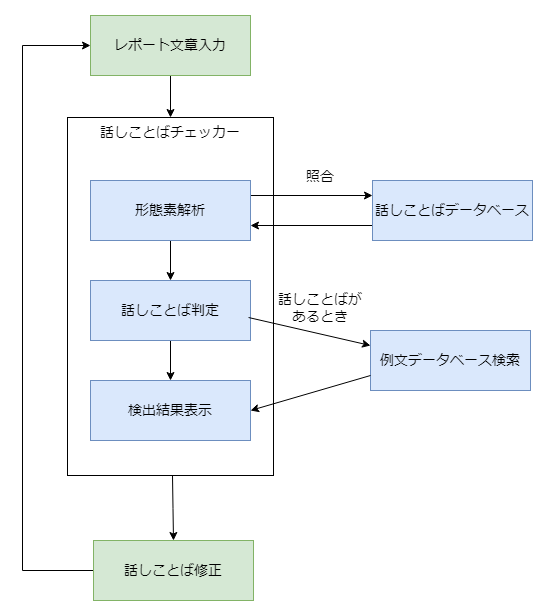
\includegraphics[width=120mm]{image/checker-flow.png}
	\caption{話しことばチェッカーの利用フロー}
	\label{checkerss-flow}
\end{figure}

\begin{figure}[H] % 別の画像貼る
	\centering
 	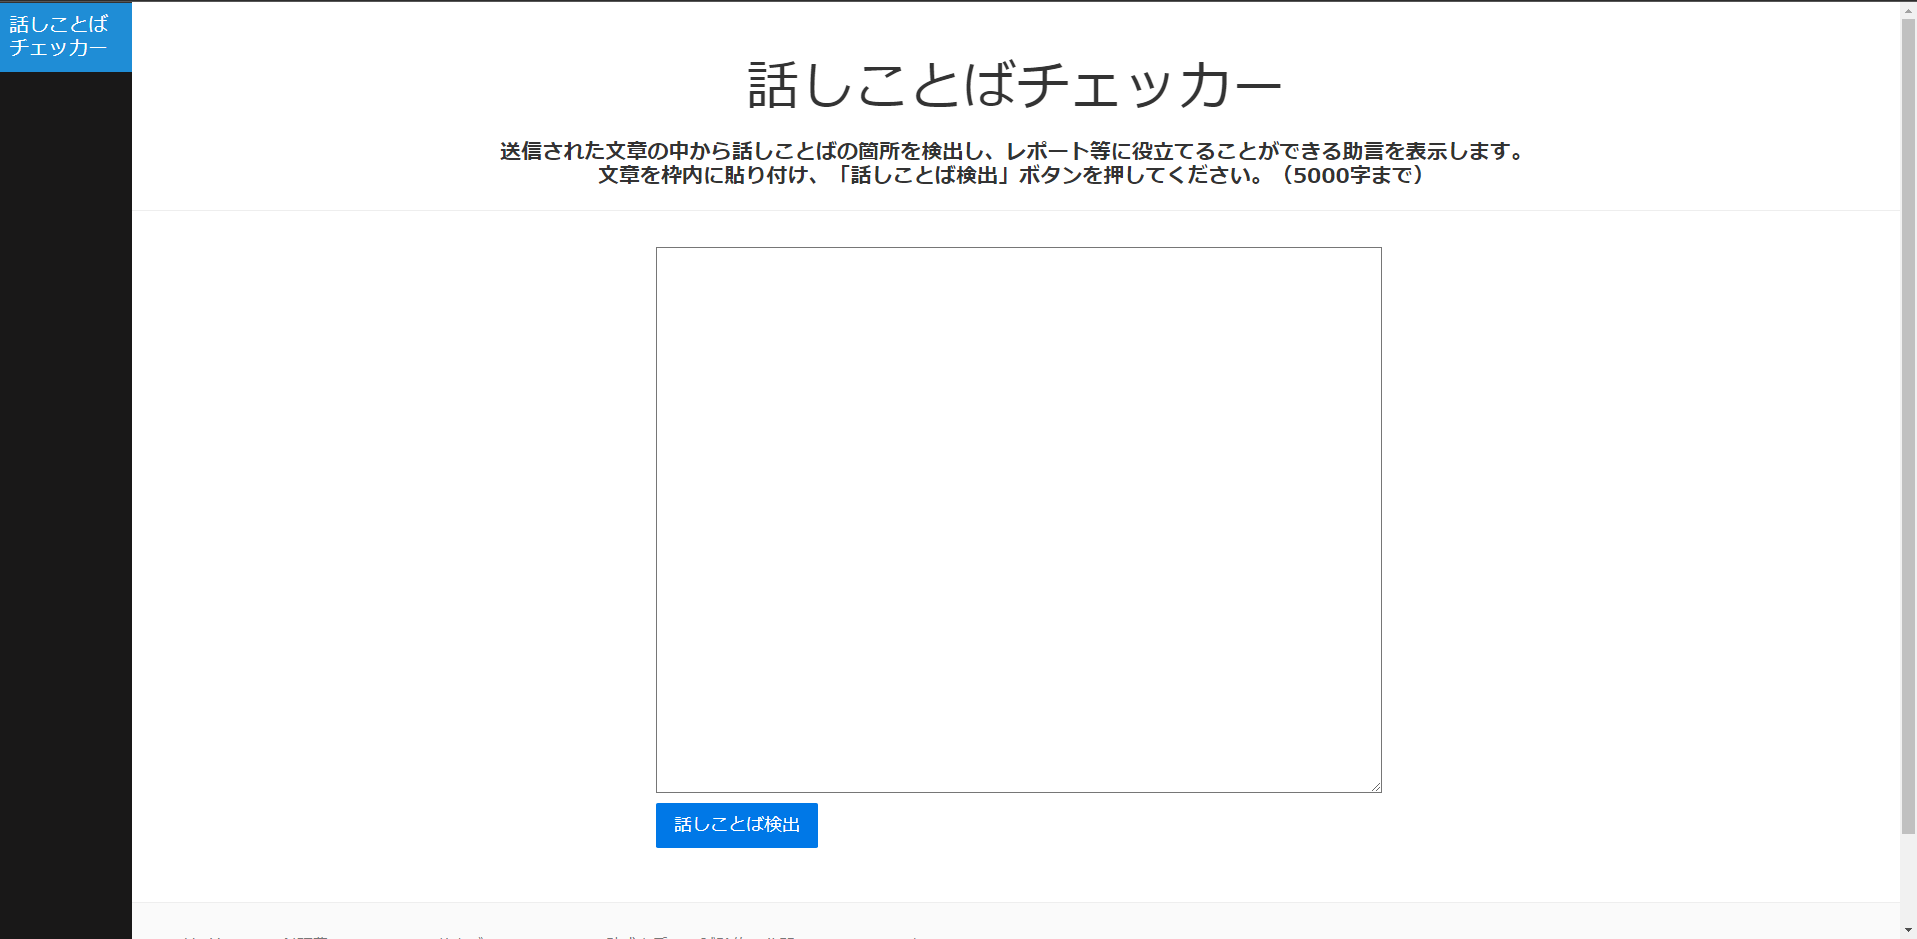
\includegraphics[width=150mm]{image/checkerss-plain.png}
	\caption{話しことばチェッカーの入力画面}
	\label{checkerss-plain}
\end{figure}

レポートなどの文章を入力し提出することで,文章中の話しことばの箇所が色付けされる.画面上で,色付けされた箇所にマウスを合わせると,書きことばへの修正例およびコメントといった推敲のための補足情報が確認できる.実際の利用画面を図\ref{checkerss-result}、図\ref{checkerss-popout}に示す.

\begin{figure}[H]
	\centering
 	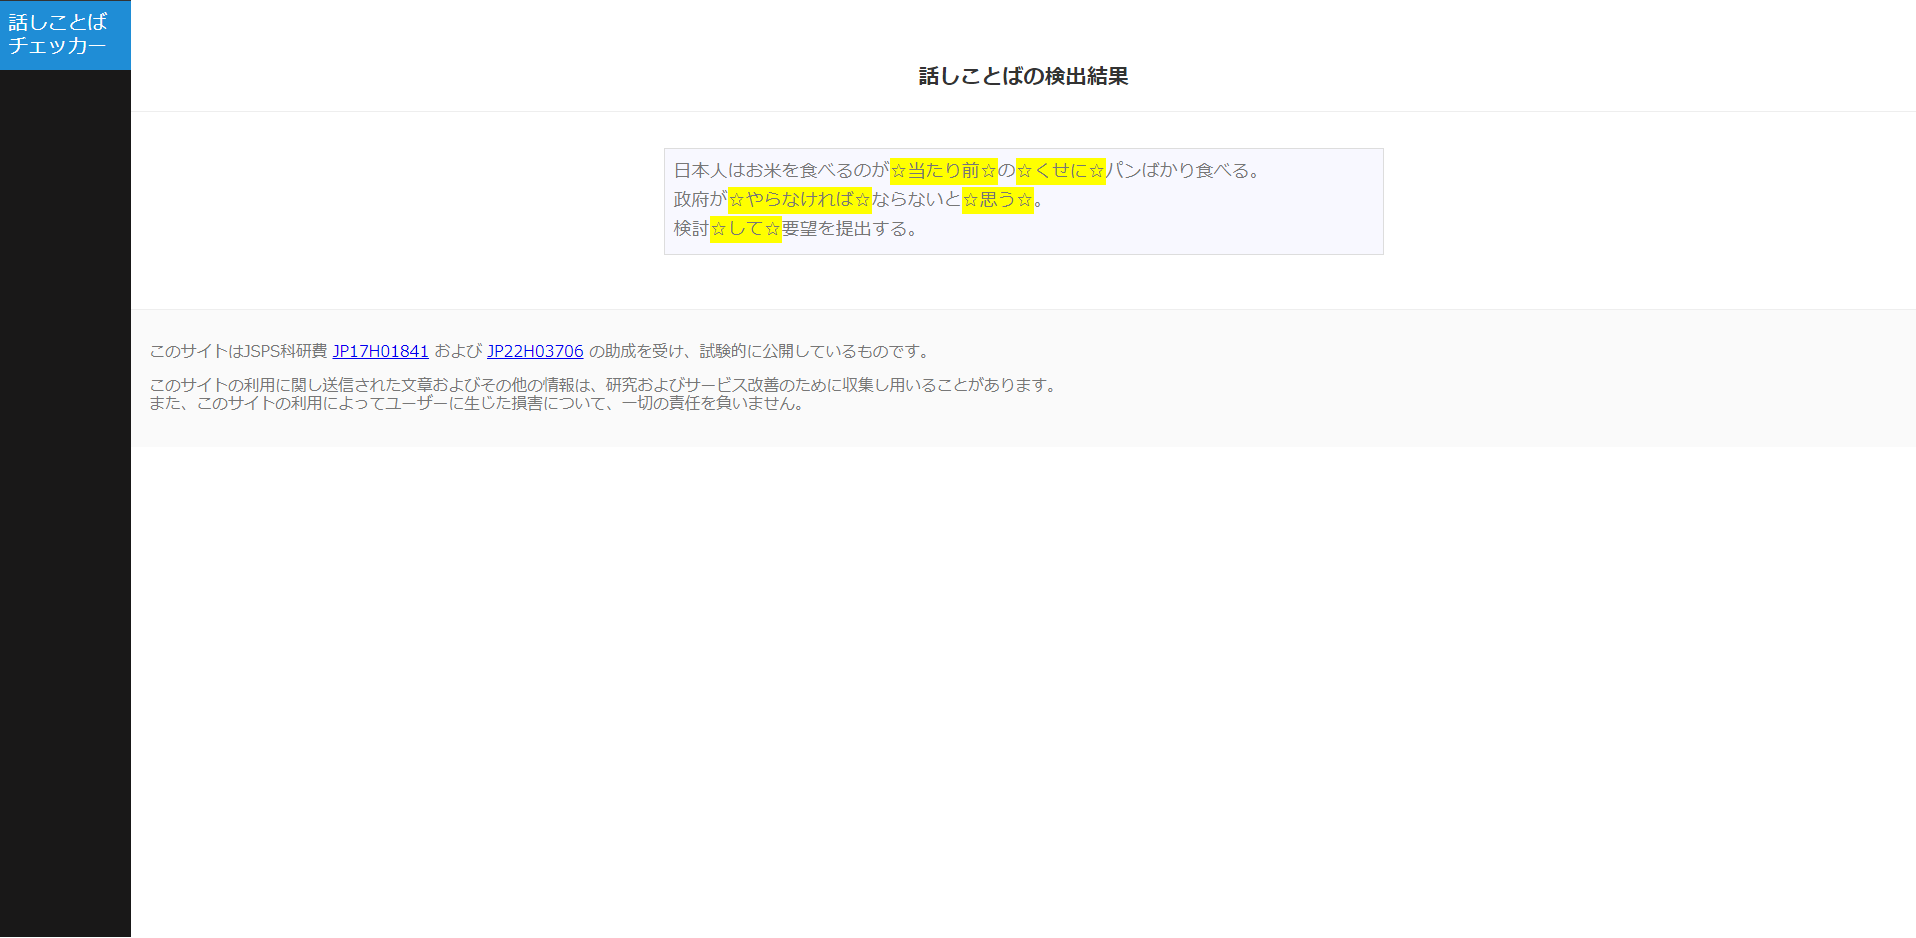
\includegraphics[width=150mm]{image/checkerss-result.png}
	\caption{話しことばチェッカーの話しことば検出画面}
	\label{checkerss-result}
\end{figure}

\begin{figure}[H]
	\centering
 	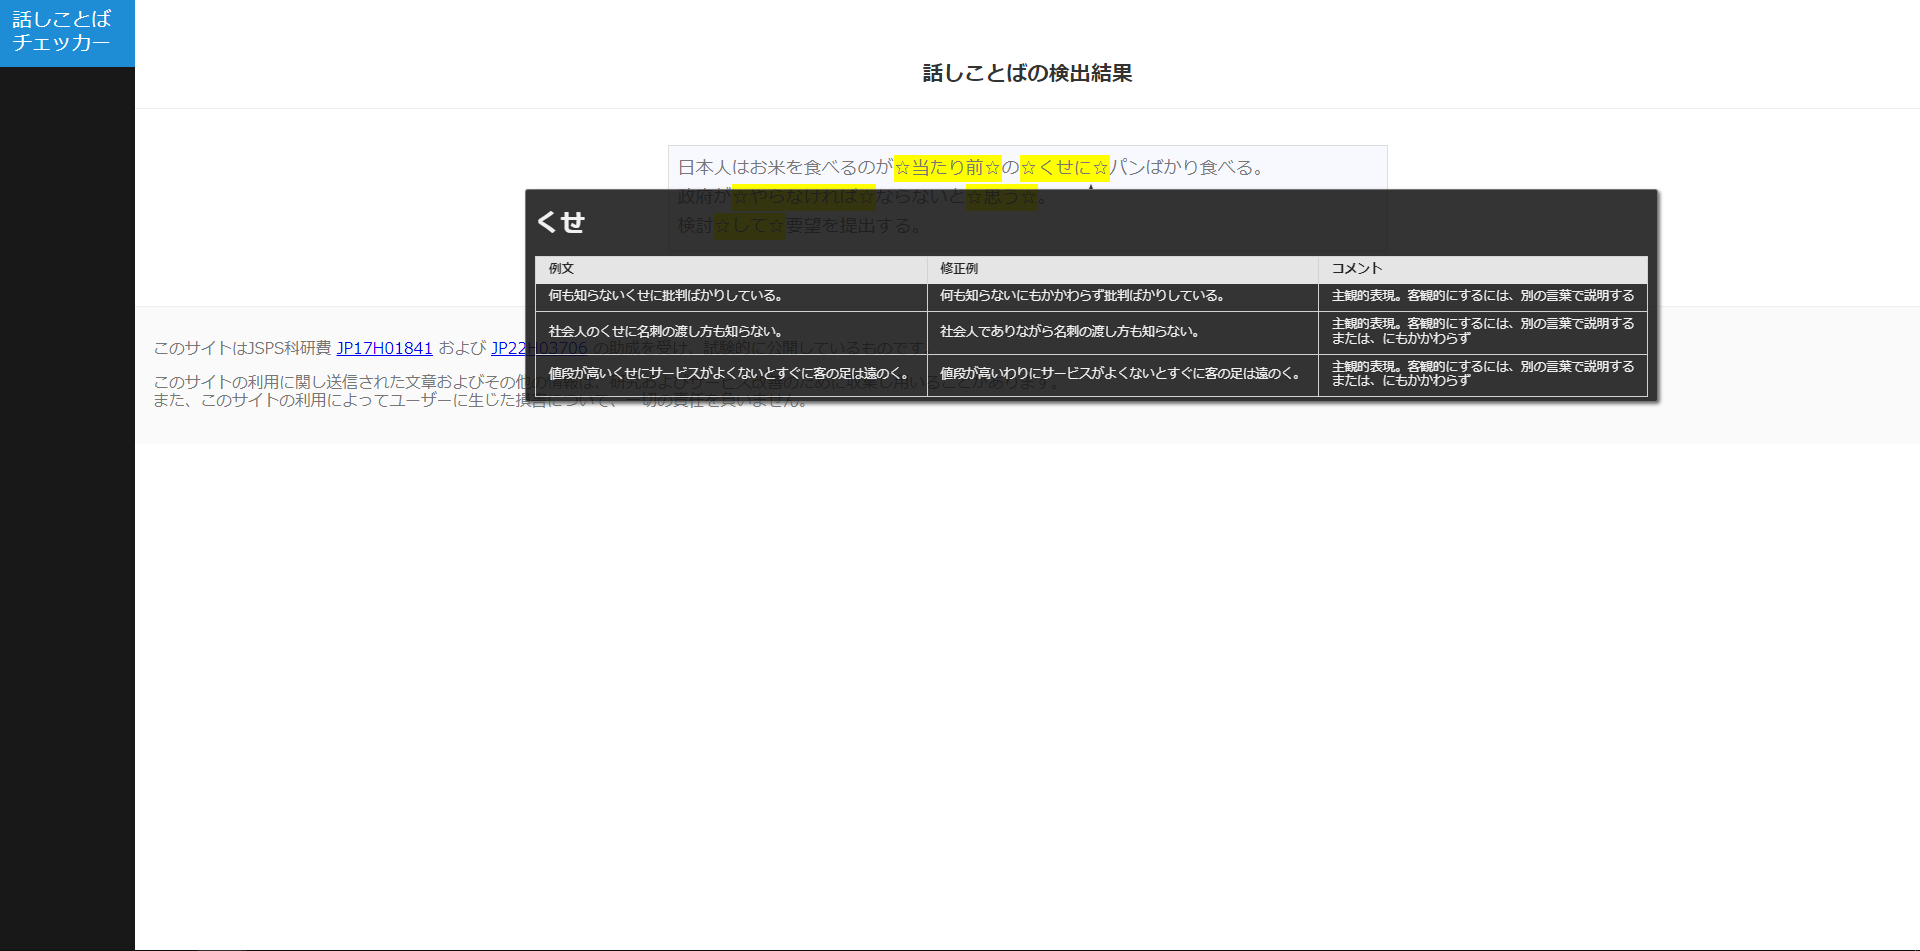
\includegraphics[width=150mm]{image/checkerss-popout.png}
	\caption{修正例などを表示している様子}
	\label{checkerss-popout}
\end{figure}

すべての話しことばのうち,INDEPENDENCE,PREFIX,SUFFIXに振り分けられている話しことばについては,現在運用している話しことばチェッカーで検出可である.一方で,COLLOCATION,OTHERに振り分けられえた話しことばは現状では不可能である.COLLOCATIONには,係り受けを伴う「~たり~たり」などの対象単語とそのほかに着目すべき単語との位置が離れているものがある.これは,話しことばの検出方式が対象単語とその前後に隣接する単語をチェックする仕様となっているためである.

現在使用されている話しことばデータベースは,話しことば事例集を基に設計されており,すべての話しことばが上記のカテゴリに分類することができる.しかし,本研究チームのこれまでの研究において,話しことばであるか書きことばであるかが不明瞭な表現が存在することがわかっており,これらの表現はカテゴリ分類を基にして話しことば検出を行っている本システムでは検出が困難である.本研究チームではこのような表現をグレーゾーンと定義している.

\section{話しことばにおけるグレーゾーン}
レポートに含まれる表現の中には,話しことばであるか書きことばであるかが不明瞭な表現が存在する.
その一例である「~てしまう」という表現は、その表現が現れる文章が主観的な文章であれば話しことばに分類されるが、客観的であれば書きことばに分類される。

例として、「家族に心配をかけたくないため、体調不良でも我慢してしまうことがある。」という文章について、文章内で主語は省略されているが、「私」などの一人称の代名詞が当てはまることが考えられる。この場合は文章が主観的なものとなるため、この「てしまう」は話しことばに分類される。

一方で、「騒がしい場所で話をすると、言葉の聞き違いが多くなってしまう。」といった一般論として述べられている文章の場合は「者」「人間」のような三人称の代名詞が当てはまることが考えられる。この場合は文章が客観的なものとなるため、この「てしまう」は書きことばに分類される。表\ref{ambiguous-ex}にグレーゾーンの例を示す。

\begin{table}[H]
\centering
\caption{グレーゾーンの例}
\begin{tabular}{|l|l|}
\hline
\multicolumn{1}{|c|}{表現} & \multicolumn{1}{c|}{例文} \\ \hline
てしまう   & \begin{tabular}[l]{@{}l@{}}アップライトピアノだと弾いている指が隠れてしまう\end{tabular} \\ \hline
残念      & \begin{tabular}[l]{@{}l@{}}楽しみにしていたイベントが中止になり残念だった\end{tabular} \\ \hline
面倒くさい & \begin{tabular}[l]{@{}l@{}}私生活では話すことを面倒くさがらずに、\\聞かれたことを真摯に答え説明する力をつけるように努力する\end{tabular} \\ \hline
厳しい     & \begin{tabular}[l]{@{}l@{}}ノルマを達成しなければ昇進は厳しい\end{tabular} \\ \hline
感じる     & \begin{tabular}[l]{@{}l@{}}人それぞれ大丈夫と感じることは異なっている\end{tabular} \\ \hline
大切      & \begin{tabular}[l]{@{}l@{}}社会で活躍できる人材を育成することも大切であると考える\end{tabular} \\ \hline
つらい     & \begin{tabular}[l]{@{}l@{}}芸能界は華やかに見えても、肉体的にも精神的にもつらい仕事がある\end{tabular} \\ \hline
\end{tabular}
\label{ambiguous-ex}
\end{table}

% 使用箇所: c3s4

2023年現在は18種類の表現がグレーゾーンに指定されている.本システムでは,グレーゾーンに指定されている特定の表現は一律で話しことばとして検出される状態になっている.表3.xに現在指定されているグレーゾーンの一覧を示す.

% グレーゾーンの一覧を載せる
